\documentclass[11pt,a4paper,fontset=fandol]{ctexart}

\usepackage{geometry}
\geometry{left=2.5cm,right=2.5cm,top=2.5cm,bottom=2.5cm}

\usepackage{booktabs}
\usepackage{tabularx}
\usepackage{listings}
\usepackage{xcolor}
\usepackage{float}
\usepackage{amsmath}
\usepackage{amssymb}
\usepackage{hyperref}
\usepackage{graphicx}

\usepackage{tikz}
\usetikzlibrary{shapes.multipart,positioning,arrows.meta,shapes.geometric,fit,calc}

\setmonofont{JetBrains Mono}

\definecolor{lightgray}{rgb}{0.95,0.95,0.95}
\definecolor{codegreen}{rgb}{0,0.6,0}
\definecolor{codegray}{rgb}{0.5,0.5,0.5}
\definecolor{codepurple}{rgb}{0.58,0,0.82}
\definecolor{backcolour}{rgb}{0.96,0.96,0.96}

\tikzset{
    entity/.style={
        draw,
        rectangle split,
        rectangle split parts=2,
        rectangle split part align={center, left},
        rounded corners=2pt,
        fill=blue!5,
        thick,
        minimum width=4.0cm,
        align=left,
        font=\huge
    },
    spatial/.style={
        draw,
        rectangle split,
        rectangle split parts=2,
        rectangle split part align={center, left},
        rounded corners=2pt,
        fill=green!5,
        thick,
        minimum width=4.0cm,
        align=left,
        font=\huge
    },
    ergroup/.style={
        draw,
        rounded corners=4pt,
        thick,
        dashed,
        inner sep=8pt
    },
    rel/.style={
        draw,
        -{Stealth[scale=0.75]},
        thick
    },
    spatialrel/.style={
        draw,
        -{Stealth[scale=0.75]},
        thick,
        dashed
    },
    flow/.style={
        draw,
        rounded corners=3pt,
        thick,
        align=center,
        minimum width=2.7cm,
        minimum height=0.9cm,
        font=\small,
        fill=blue!5
    },
    flowcheck/.style={
        flow,
        diamond,
        aspect=2.1,
        inner sep=1pt,
        fill=orange!10
    },
    flowstore/.style={
        flow,
        fill=green!8
    },
    flowbad/.style={
        flow,
        fill=red!6
    },
    flowline/.style={
        draw,
        -{Stealth[scale=0.9]},
        thick
    },
    line/.style={
        draw,
        -{Stealth[scale=0.8]},
        thick
    },
    relation/.style={
        draw,
        diamond,
        aspect=1.6,
        fill=blue!5,
        thick,
        minimum width=1.8cm,
        minimum height=1.0cm,
        align=center,
        font=\LARGE\bfseries,
        inner sep=2pt
    },
    relation_spatial/.style={
        draw,
        diamond,
        aspect=1.6,
        fill=green!5,
        thick,
        dashed,
        minimum width=1.8cm,
        minimum height=1.0cm,
        align=center,
        font=\LARGE\bfseries,
        inner sep=2pt
    },
    rel_line/.style={
        draw,
        thick
    },
    spatial_rel_line/.style={
        draw,
        thick,
        dashed
    }
}

\lstset{
    backgroundcolor=\color{backcolour},   
    commentstyle=\color{codegreen},
    keywordstyle=\color{blue},
    numberstyle=\tiny\color{codegray},
    stringstyle=\color{codepurple},
    basicstyle=\ttfamily\footnotesize,
    breakatwhitespace=false,         
    breaklines=true,                 
    captionpos=b,                    
    keepspaces=true,                 
    numbers=left,                    
    numbersep=5pt,                  
    showspaces=false,                
    showstringspaces=false,
    showtabs=false,                  
    tabsize=2
}

\begin{document}
\nocite{*}

\begin{titlepage}
    \centering
    \vspace*{1.5cm}
    
    
\includegraphics[width=0.7\textwidth]{figs/img14.png}
    
    \vspace{2cm}
    
    {\Large
    \renewcommand{\arraystretch}{1.5}
    \begin{tabular}{r@{\extracolsep{0.2em}}c}
        \textbf{课程名称：} & \underline{\makebox[280pt][c]{数据库原理及应用}} \\
        \textbf{作业题目：} & \underline{\makebox[280pt][c]{比利时与荷兰地区大型电子音乐节运营}} \\
        & \underline{\makebox[280pt][c]{与空间选址数据库设计与 PostGIS 分析报告}} \\
        \textbf{授课教师：} & \underline{\makebox[280pt][c]{张昆}} \\
        \textbf{学\qquad 院：} & \underline{\makebox[280pt][c]{地理科学学院}} \\
        \textbf{专\qquad 业：} & \underline{\makebox[280pt][c]{地理信息科学}} \\
        \textbf{学\qquad 号：} & \underline{\makebox[280pt][c]{10233903433}} \\
        \textbf{姓\qquad 名：} & \underline{\makebox[280pt][c]{胡盛扉}} \\
    \end{tabular}
    }
    
    \vfill
    
    {\Large 2026 年 7 月}
    \vspace*{3em}
\end{titlepage}
\newpage

\tableofcontents
\newpage


\section{项目概述}

比利时与荷兰地区的大型户外电子音乐节在国际上享有盛誉，每年吸引数十万名全球观众。此类大型活动的举办同时具备复杂的业务运营属性与强烈的空间规划约束。一方面，在运营层面，主办方需要对音乐节品牌、年度届次、场地设施、演出舞台、艺人阵容、演出节目块以及门票销售等业务实体进行精细化管理；另一方面，在空间层面，由于此类活动具有高噪声、高人员流动性以及大面积占用等特点，选址必须在便利的交通可达性、充足的市场人口覆盖、严格的生态环境保护与控制对周边居民噪声干扰之间取得平衡。

本项目旨在构建一个综合性的 PostgreSQL 扩展 PostGIS 数据库系统，将传统的业务关系层与先进的空间分析层融合在统一的数据架构中。我们选取了该地区最具代表性的三个电子音乐节作为具体研究对象，其基础信息如表\ref{tab:festivals}所示。

\begin{table}[H]
\centering
\caption{项目分析对象概览}
\label{tab:festivals}
\begin{tabular}{lccc}
\toprule
音乐节 & 届次 & 国家 & 场地 \\
\midrule
Tomorrowland & 2025 & 比利时 & De Schorre, Boom \\
Defqon.1 & 2025 & 荷兰 & Walibi Holland event grounds, Biddinghuizen \\
Awakenings Summer Festival & 2025 & 荷兰 & Beekse Bergen, Hilvarenbeek \\
\bottomrule
\end{tabular}

\end{table}

项目实现了以下核心目标：首先，建立高度规范化的音乐节运营关系模型，重点解决多艺人合作演出、多销售阶段门票定价等复杂业务场景；其次，设计多指标空间选址评分模型，利用空间叠加与距离分析计算场地综合得分；最后，通过真实案例的空间距离匹配，验证模型的选址结果是否与现实举办场地相契合，从而形成理论设计、计算实现与现实场景验证的完整闭环。

\section{数据来源与真实性分层}

\subsection{数据来源}

本项目的数据来源涵盖空间地理数据与官方业务数据两大类。在空间层面，\textbf{候选场地与敏感设施}通过 OpenStreetMap (OSM) 接口与 Overpass API 提取区域内的公园、草地、休闲场地作为候选地，同时提取学校、医院、养老院及居民区等噪声敏感设施点位；\textbf{交通枢纽}利用 OurAirports 开放数据及 OSM 提取民用机场、火车站和公交枢纽，用于评估场地交通可达性；\textbf{生态保护区}采用欧洲环境署 (EEA) 提供的 Natura 2000 矢量边界，作为生态红线避让约束；\textbf{人口网格}采用欧盟统计局 (Eurostat/GISCO) 发布的 2021 版 1公里网格人口数据，用于计算候选场地周边的人口覆盖度及潜在噪声受影响人口。

在业务层面，项目从多个渠道采集了三大音乐节的真实运营数据。\textbf{Tomorrowland} 通过 Wayback Machine 检索并下载了 2025 年官方 Timetable 和票价页面的结构化快照，获取了完整的舞台、艺人、演出时刻及多阶段门票报价数据；\textbf{Awakenings} 对当前官方 Shop API 执行了深层抓包审计，获取了 2025 年活动基本事实以及住宿套餐价格；\textbf{Defqon.1} 通过官方历史页面快照确认了 2025 年的举办日期与购票入口，但由于历史报价数据未在页面直接渲染，普通门票价格在此作留空处理。

\subsection{数据真实性分层与治理体系}

在多源数据融合过程中，为了保证核心业务表的纯洁性，本项目建立了严格的数据真实性分层治理体系。所有采集到的原始数据首先导入无外键约束的 Staging 暂存表中，经过年份、语义及置信度审计后，符合高置信度要求的数据才提升（Promote）至正式业务表中；对于无法确认的通用候选数据，则保留在暂存表中不作提升。具体分层数据特征如表\ref{tab:data_quality}所示。

\begin{table}[H]
\centering
\caption{数据真实性分层与治理体系}
\label{tab:data_quality}
\begin{tabularx}{\textwidth}{lXX}
\toprule
数据级别 & 典型字段与要素 & 处理与写入策略 \\
\midrule
官方真实数据 & 演出时刻表、舞台空间点位、Natura 2000 边界 & 经 Staging 暂存表审计后直接写入正式业务表。 \\
公开空间数据 & OSM 候选地边界、学校与医院位置、人口网格 & 统一投影转换至 EPSG:3035 并建立 GiST 空间索引。 \\
模拟估计数据 & 预计观众规模、阶段门票配额、舞台估计容量、估计观众密集度 & 允许为空，或在报告中明确标注为估计值，不影响物理外键完整性。 \\
\bottomrule
\end{tabularx}
\end{table}

\section{数据库逻辑结构与约束设计}

\subsection{技术环境与空间基准}

本系统基于 PostgreSQL 18 数据库管理系统配合 PostGIS 扩展模块实现。为了确保在欧洲尺度下进行高精度的面积与距离计算，所有空间几何数据统一采用扩展的欧洲 LAEA 投影坐标系，即 EPSG:3035 空间坐标系。该坐标系基于米和平方米单位，可避免常规经纬度坐标系在距离缓冲区计算中产生的变形误差。

\subsection{数据表结构逻辑设计与 E-R 图}

本系统共设计了 18 张表。业务关系层主要关注核心运营实体，而空间分析层则专注于地理空间分析实体，其整体逻辑 E-R 关系图如图\ref{fig:er_diagram}所示。

\begin{figure}[H]
\centering
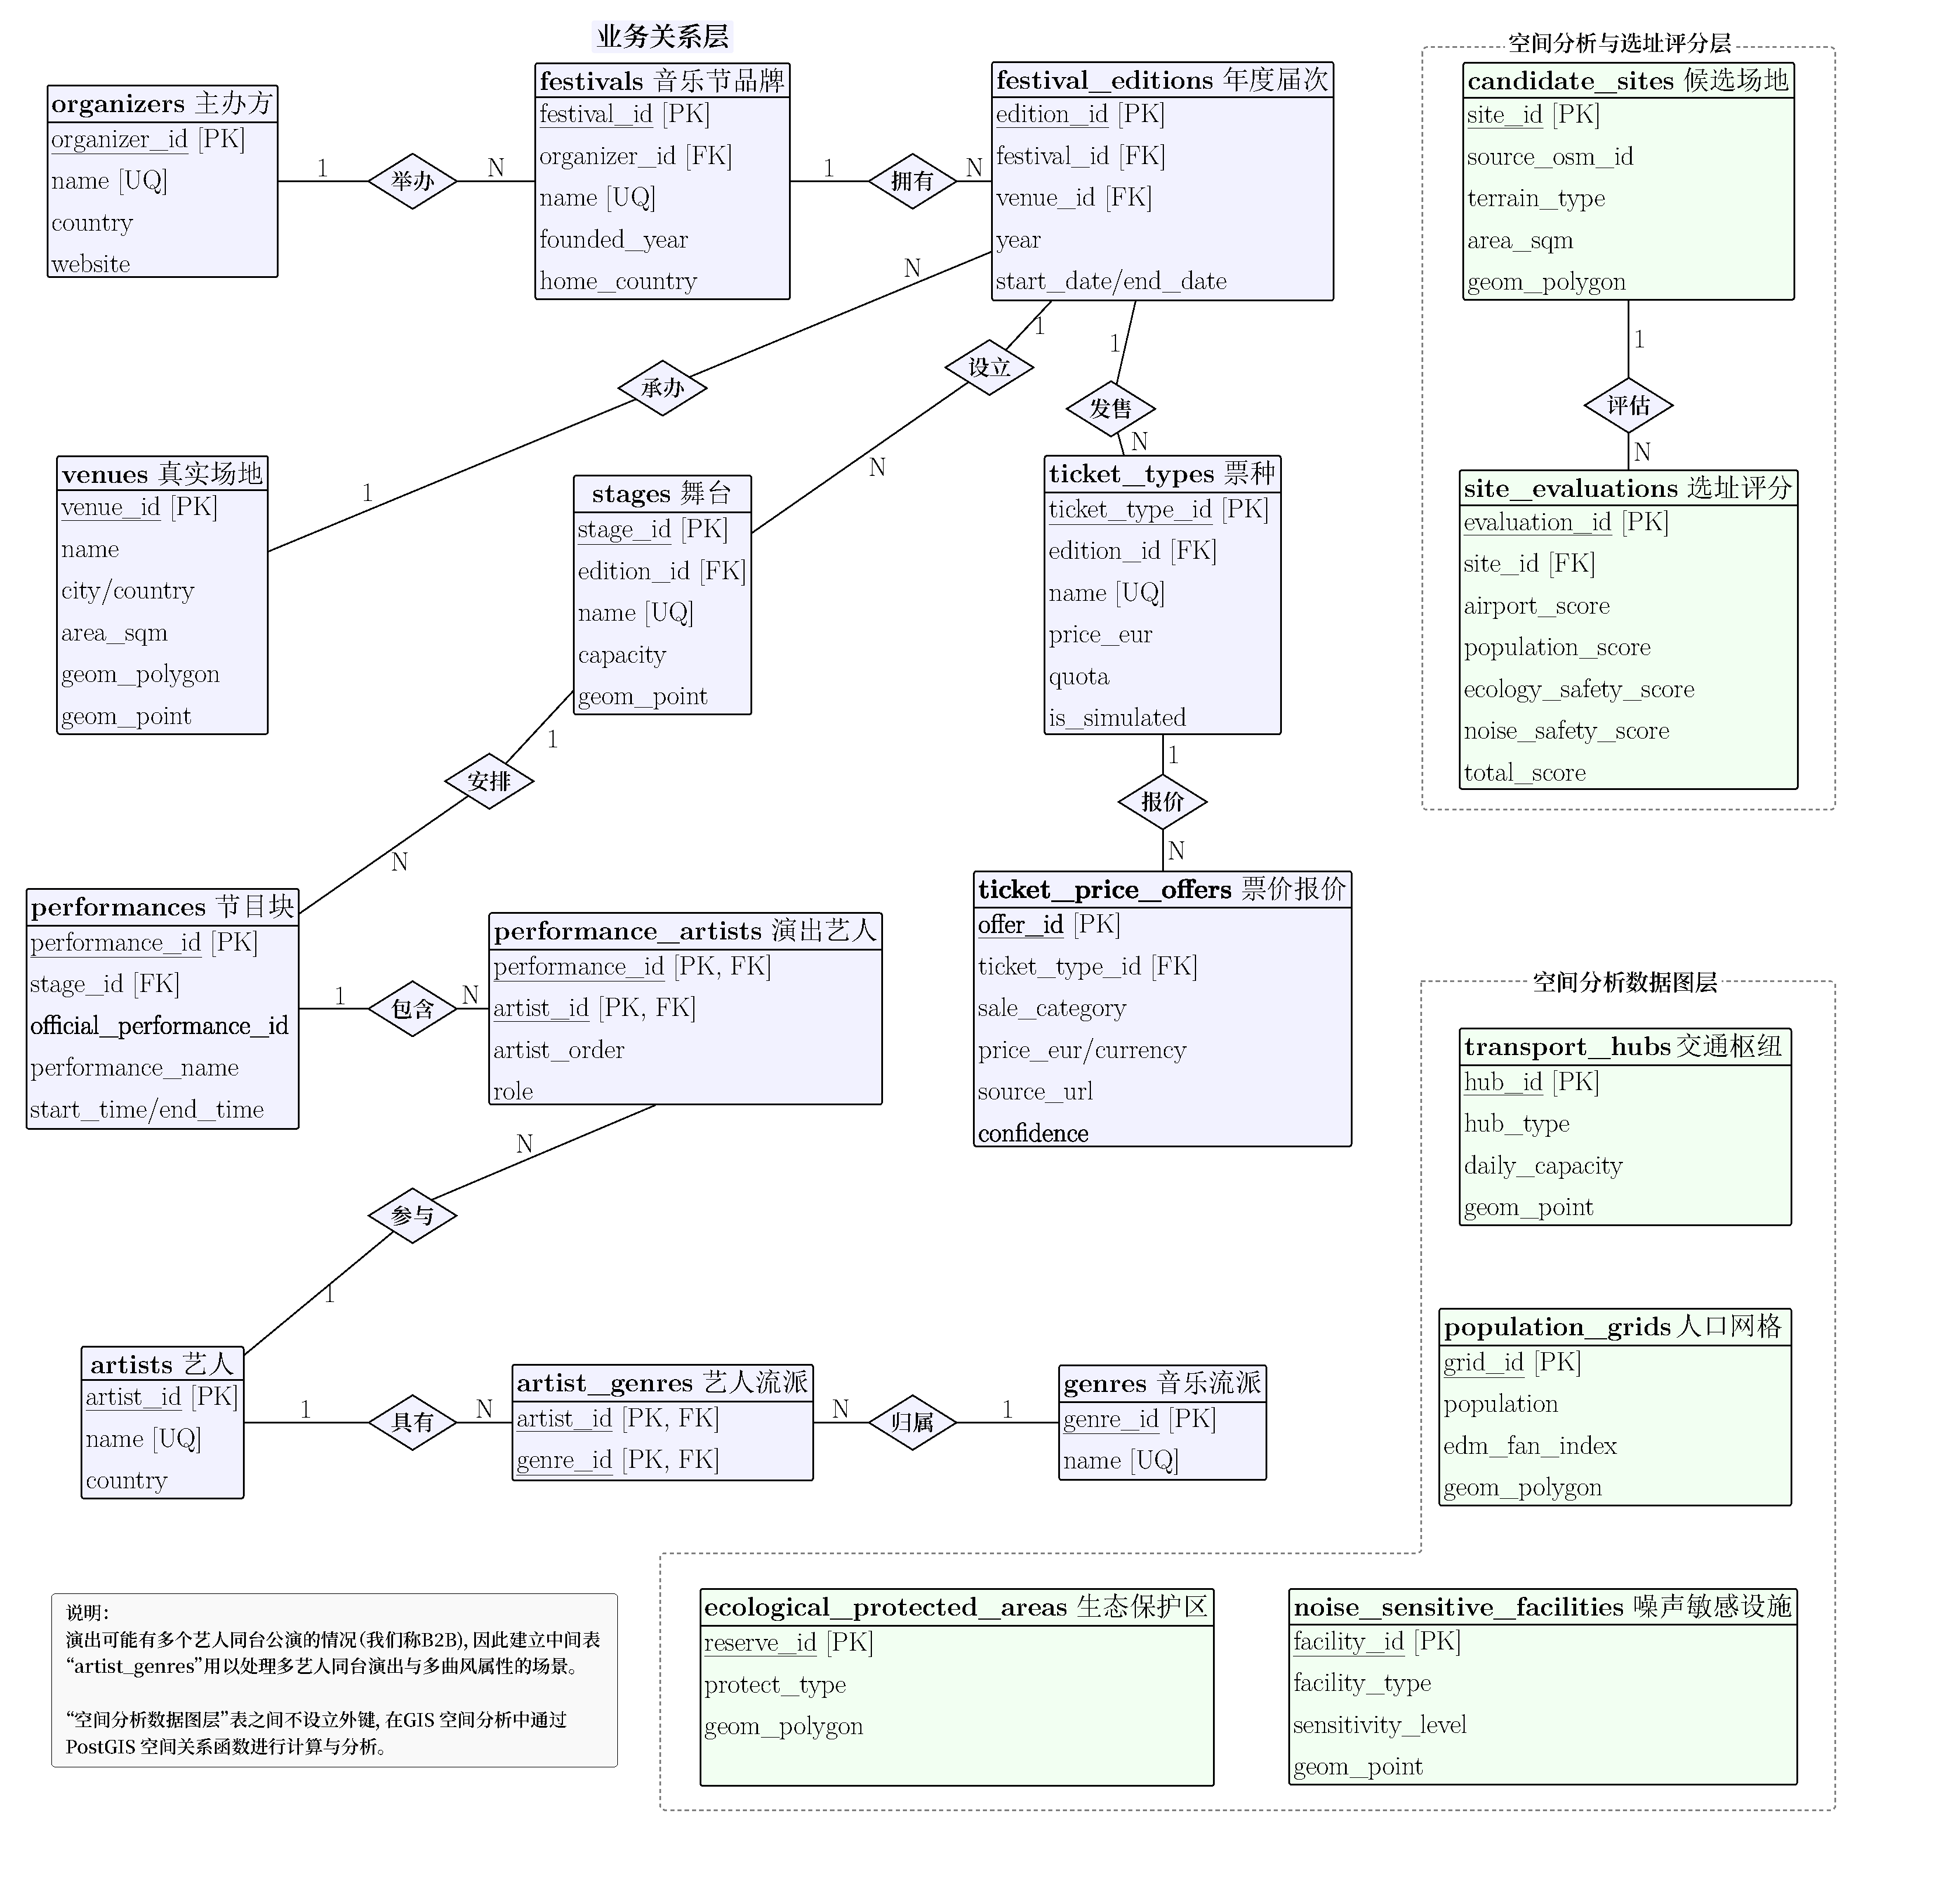
\includegraphics[width=\textwidth]{figs/ERdiagram.pdf}
\caption{电子音乐节业务管理与空间分析数据库 E-R 关系图}
\label{fig:er_diagram}
\end{figure}

\subsection{复杂场景的规范化建模优化}

在逻辑结构设计中，针对现实运营的复杂特性，本项目实施了两项规范化改进：

第一，\textbf{多艺人演出联合建模}：在主流音乐节中，多名艺人同台演出或者以合作形式进行表演的情况极为普遍。若在 \texttt{performances} 表中直接记录单一艺人主键，将违背关系模式的规范化要求。为此，本项目引入了多对多关联表 \texttt{performance\_artists}，通过 \texttt{artist\_order} 字段维护艺人出场顺序，通过 \texttt{role} 字段明确其演出角色，从而有效解决了多人同台演出的数据结构表达。

第二，\textbf{多阶段门票报价建模}：门票销售通常包含内部预售、Belgian Pre-Sale、Worldwide Pre-Sale 以及 Worldwide Sale 等多个销售波次。同一票种在不同阶段的官方定价差异显著。传统设计在 \texttt{ticket\_types} 表中仅设置单一价格字段，无法记录完整的价格变动。为此，本项目抽象出 \texttt{ticket\_price\_offers} 报价细分表，将具体报价与票种主表剥离，完整保留了多销售阶段的票价血缘。

\subsection{范式检查与完整性约束}

经评估，所设计的业务关系模式完全满足第三范式的要求，排除了非主属性对码的传递依赖和部分依赖。为保障数据库底层的数据完整性与空间正确性，我们配置了严格的检查约束与空间索引。建表与约束 DDL 核心代码如下所示：

\begin{lstlisting}[language=SQL]
-- 1. 创建空间扩展
CREATE EXTENSION IF NOT EXISTS postgis;

-- 2. 真实场地表定义与空间有效性检查
CREATE TABLE venues (
    venue_id integer GENERATED BY DEFAULT AS IDENTITY PRIMARY KEY,
    name varchar(160) NOT NULL,
    city varchar(100) NOT NULL,
    country varchar(80) NOT NULL,
    area_sqm numeric(14,2) CHECK (area_sqm IS NULL OR area_sqm > 0),
    data_source text,
    geom_polygon geometry(MultiPolygon, 3035),
    geom_point geometry(Point, 3035) NOT NULL,
    CONSTRAINT chk_venues_geom_polygon_valid
        CHECK (geom_polygon IS NULL OR (ST_IsValid(geom_polygon) AND ST_SRID(geom_polygon) = 3035)),
    CONSTRAINT chk_venues_geom_point_valid
        CHECK (ST_IsValid(geom_point) AND ST_SRID(geom_point) = 3035)
);

-- 3. 候选场地表定义与物理约束
CREATE TABLE candidate_sites (
    site_id integer GENERATED BY DEFAULT AS IDENTITY PRIMARY KEY,
    name varchar(160) NOT NULL,
    source_osm_id varchar(80),
    terrain_type varchar(80) NOT NULL,
    area_sqm numeric(14,2) NOT NULL,
    daily_cost numeric(12,2) CHECK (daily_cost IS NULL OR daily_cost >= 0),
    data_source text,
    is_manual_sample boolean NOT NULL DEFAULT true,
    geom_polygon geometry(MultiPolygon, 3035) NOT NULL,
    CONSTRAINT chk_site_area CHECK (area_sqm >= 50000),
    CONSTRAINT chk_site_geom_valid CHECK (ST_IsValid(geom_polygon) AND ST_SRID(geom_polygon) = 3035)
);

-- 4. 建立空间 GiST 索引以加速拓扑计算
CREATE INDEX idx_venues_geom_polygon ON venues USING gist (geom_polygon);
CREATE INDEX idx_venues_geom_point ON venues USING gist (geom_point);
CREATE INDEX idx_candidate_sites_geom ON candidate_sites USING gist (geom_polygon);
CREATE INDEX idx_transport_hubs_geom ON transport_hubs USING gist (geom_point);
CREATE INDEX idx_population_grids_geom ON population_grids USING gist (geom_polygon);
CREATE INDEX idx_protected_areas_geom ON ecological_protected_areas USING gist (geom_polygon);
CREATE INDEX idx_noise_sensitive_geom ON noise_sensitive_facilities USING gist (geom_point);

-- 5. 建立业务查询索引以加速个性化 timetable 推荐
CREATE EXTENSION IF NOT EXISTS pg_trgm;
CREATE INDEX idx_performances_start_time ON performances(start_time);
CREATE INDEX idx_performances_business_day
    ON performances(((start_time - interval '5 hours')::date));
CREATE INDEX idx_genres_name_trgm ON genres USING gin (name gin_trgm_ops);
\end{lstlisting}

\section{数据治理与清洗流程}

\subsection{暂存与分层治理流}

为了防止不受信任的网页抓取字段或者年份不匹配的脏数据直接污染核心业务表，项目引入了数据暂存分层治理架构。外部源数据首先导入到无强约束的 Staging 暂存表中，随后通过专用的提升脚本执行完整性与置信度审计，最后才注入正式的关系表中，具体流程如图\ref{fig:workflow}所示。

\begin{figure}[H]
    \centering
    \resizebox{\textwidth}{!}{%
    \begin{tikzpicture}[node distance=1.05cm and 1.15cm]
        \node[flow] (raw) {原始数据源\\HTML / JSON / CSV / GeoJSON};
        \node[flowstore, right=of raw] (archive) {原始文件归档\\保留来源 URL 与时间戳};
        \node[flow, right=of archive] (parse) {脚本解析\\Python / PowerShell};
        \node[flowstore, right=of parse] (staging) {Staging 暂存表\\候选值不直接入核心表};

        \node[flowcheck, below=of staging] (audit) {来源、年份、字段语义\\与置信度审计};
        \node[flowstore, left=of audit] (promote) {Promote SQL\\写入正式业务表};
        \node[flowbad, right=of audit] (hold) {保留为候选\\或记录不可得原因};

        \node[flowstore, below=of promote] (core) {核心关系表\\业务数据};
        \node[flowstore, below=of hold] (spatial) {空间分析表\\PostGIS 几何与索引};
        \node[flow, below=1.05cm of audit] (export) {视图与导出\\QGIS / CSV / 报告表格};

        \path[flowline] (raw) -- (archive);
        \path[flowline] (archive) -- (parse);
        \path[flowline] (parse) -- (staging);
        \path[flowline] (staging) -- (audit);
        \path[flowline] (audit) -- node[above]{可信} (promote);
        \path[flowline] (audit) -- node[above]{不可归属} (hold);
        \path[flowline] (promote) -- (core);
        \path[flowline] (hold) -- (spatial);
        \path[flowline] (core) -- (export);
        \path[flowline] (spatial) -- (export);
    \end{tikzpicture}%
    }
    \caption{分层数据治理与清洗提升流程}
    \label{fig:workflow}
\end{figure}

\subsection{历史演示样本清理}

项目数据治理的一项关键成果是彻底剔除了早期手工构建的虚拟过渡样本。对于保护区、敏感点与交通节点，原有的近似多边形被完全删除，取而代之的是由欧洲环境署和开放街图提供的真实规范数据。数据清洗脚本中通过条件语句对过渡样本进行了清除，保证了分析库的纯洁性：

\begin{lstlisting}[language=SQL]
-- 清理被正式公开数据所替换的早期演示手工样本
DELETE FROM candidate_sites WHERE is_manual_sample = true AND site_id NOT IN (
    SELECT DISTINCT site_id FROM site_evaluations
);
DELETE FROM ecological_protected_areas WHERE data_source = 'manual_seed';
DELETE FROM noise_sensitive_facilities WHERE data_source = 'manual_seed';
DELETE FROM transport_hubs WHERE data_source = 'manual_seed';
\end{lstlisting}

\section{基于 PostGIS 的多准则选址模型与空间分析}

\subsection{选址评估指标体系与数学表达}

选址评估模型共考虑四个分项评估维度与最终的综合选址得分，其值域均映射至 $0 \sim 100$ 的区间，物理释义分别如下：
\begin{itemize}
    \item \textbf{交通可达性 ($S_{\text{airport}}$)}：以 100 公里为基准，距离最近机场越近得分越高，超出该范围计 0 分。
    \item \textbf{市场人口覆盖 ($S_{\text{population}}$)}：计算周边 25 公里范围内的人口网格总数，采用电子音乐兴趣指数进行加权累加，并与区域最大加权人口进行归一化映射。
    \item \textbf{生态安全 ($S_{\text{ecology}}$)}：评估对 Natura 2000 生态保护区的避让程度，每远离 1 公里得 1 分，100 公里即得满分，直接相交的场地计 0 分。
    \item \textbf{噪声防范安全 ($S_{\text{noise}}$)}：评估对学校、医院等高敏感噪声点的影响，每远离 100 米得 1 分，10 公里即得满分。
    \item \textbf{综合选址得分 ($S_{\text{total}}$)}：由上述四项指标加权求和得出，分配的权重分别为：交通可达性占比 30\%、市场人口覆盖占比 25\%、噪声防范安全占比 25\%、生态安全占比 20\%。
\end{itemize}

各维度的数学计算公式与最终的综合选址评分加权公式依次定义如下：
\begin{align}
    S_{\text{airport}} &= \max\left(0, \min\left(100, 100 - \frac{d_{\text{airport}}(\text{m})}{1000.0}\right)\right) \\
    S_{\text{population}} &= \min\left(100, \frac{\sum (P_i \times I_i)}{P_{\text{max\_weighted}}} \times 100\right) \\
    S_{\text{ecology}} &= \max\left(0, \min\left(100, \frac{d_{\text{ecology}}(\text{m})}{1000}\right)\right) \\
    S_{\text{noise}} &= \max\left(0, \min\left(100, \frac{d_{\text{noise}}(\text{m})}{100.0}\right)\right) \\
    S_{\text{total}} &= 0.30 \times S_{\text{airport}} + 0.25 \times S_{\text{population}} + 0.20 \times S_{\text{ecology}} + 0.25 \times S_{\text{noise}}
\end{align}

为保证选址评分可以由数据库自动复算，项目将四类空间指标写成一条 PostGIS 查询。该查询综合使用 \texttt{ST\_Distance}、\texttt{ST\_DWithin}、GiST 最近邻排序算子 \texttt{<->} 以及人口网格空间连接，最终生成候选场地的交通、人口、生态与噪声分项得分。核心 SQL 如下：

\begin{lstlisting}[language=SQL]
WITH metrics AS (
    SELECT
        s.site_id,
        COALESCE(airport.nearest_airport_m, 1000000) AS nearest_airport_m,
        COALESCE(sensitive.nearest_sensitive_m, 1000000) AS nearest_sensitive_m,
        COALESCE(ecology.nearest_ecology_m, 1000000) AS nearest_ecology_m,
        COALESCE(pop.weighted_population_25km, 0) AS weighted_population_25km
    FROM candidate_sites s
    LEFT JOIN LATERAL (
        SELECT ST_Distance(s.geom_polygon, h.geom_point) AS nearest_airport_m
        FROM transport_hubs h
        WHERE h.hub_type = 'airport'
        ORDER BY s.geom_polygon <-> h.geom_point
        LIMIT 1
    ) airport ON true
    LEFT JOIN LATERAL (
        SELECT ST_Distance(s.geom_polygon, n.geom_point) AS nearest_sensitive_m
        FROM noise_sensitive_facilities n
        WHERE n.sensitivity_level >= 4
        ORDER BY s.geom_polygon <-> n.geom_point
        LIMIT 1
    ) sensitive ON true
    LEFT JOIN LATERAL (
        SELECT ST_Distance(s.geom_polygon, e.geom_polygon) AS nearest_ecology_m
        FROM ecological_protected_areas e
        ORDER BY s.geom_polygon <-> e.geom_polygon
        LIMIT 1
    ) ecology ON true
    LEFT JOIN LATERAL (
        SELECT SUM(g.population * g.edm_fan_index) AS weighted_population_25km
        FROM population_grids g
        WHERE g.geom_polygon && ST_Expand(s.geom_polygon, 25000)
          AND ST_DWithin(s.geom_polygon, g.geom_polygon, 25000)
    ) pop ON true
),
scored AS (
    SELECT
        site_id,
        ROUND(GREATEST(0, LEAST(100, 100 - nearest_airport_m / 1000.0))::numeric, 2) AS airport_score,
        ROUND(
            CASE WHEN MAX(weighted_population_25km) OVER () = 0 THEN 0
                 ELSE GREATEST(0, LEAST(100, weighted_population_25km
                      / MAX(weighted_population_25km) OVER () * 100))
            END::numeric, 2
        ) AS population_score,
        ROUND(GREATEST(0, LEAST(100, nearest_ecology_m / 1000.0))::numeric, 2) AS ecology_safety_score,
        ROUND(GREATEST(0, LEAST(100, nearest_sensitive_m / 100.0))::numeric, 2) AS noise_safety_score
    FROM metrics
)
SELECT
    site_id,
    airport_score,
    population_score,
    ecology_safety_score,
    noise_safety_score,
    ROUND((0.30 * airport_score + 0.25 * population_score
         + 0.20 * ecology_safety_score + 0.25 * noise_safety_score)::numeric, 2) AS total_score
FROM scored
ORDER BY total_score DESC;
\end{lstlisting}

基于 PostGIS 的联合查询计算，提取出了综合评分前五名的候选场地，详细评分组成如表\ref{tab:top_sites}所示。

\begin{table}[H]
\centering
\caption{综合评分前五名候选场地评分分解}
\label{tab:top_sites}
\begin{tabular}{lcccccc}
\toprule
排名 & 候选场地 & 总分 & 交通得分 & 人口得分 & 噪声安全 & 生态安全 \\
\midrule
1 & Molecaten Parc Flevostrand & 54.14 & 89.21 & 20.10 & 89.33 & 0.10 \\
2 & Tivolipark & 51.72 & 87.90 & 100.00 & 0.40 & 1.25 \\
3 & De Schorre & 49.31 & 88.18 & 82.65 & 4.25 & 5.66 \\
4 & Domein Roosendael & 48.93 & 87.05 & 87.26 & 3.51 & 0.60 \\
5 & Park Fort Liezele & 48.90 & 84.77 & 91.28 & 2.58 & 0.01 \\
\bottomrule
\end{tabular}
\end{table}

分析表\ref{tab:top_sites}的数据可以发现，当前综合评分最高的 Molecaten Parc Flevostrand 在交通可达性与噪声安全之间取得了较好的平衡，因此总分位列第一。Tivolipark、De Schorre、Domein Roosendael 与 Park Fort Liezele 虽然在人口市场覆盖维度上表现突出，但噪声安全和生态安全得分普遍较低，说明这些地点更接近城市建成区、学校或生态敏感区域。该结果反映出大型音乐节选址并非单纯追求人口覆盖，而是在交通便利性、市场规模与环境扰动风险之间进行权衡。

\begin{figure}[H]
    \centering
    \includegraphics[width=\linewidth]{figs/candidate_scores2.png}
    \caption{比荷卢地区三大电子音乐节周边候选区域综合选址评分分级地图}
    \label{fig:qgis_candidate_scores}
    \par\vspace{3pt}
    {\footnotesize 注：子图 (a)、(b)、(c) 分别对应 Tomorrowland (比利时 Boom)、Defqon.1 (荷兰 Biddinghuizen) 与 Awakenings (荷兰 Hilvarenbeek) 音乐节周边的候选场地分布。图例展示了经多准则空间模型计算后的综合得分（29.41 - 54.14），采用自然断点法分为七级，颜色由红色（低分，代表选址劣势明显）向蓝色（高分，代表选址优势突出）过渡。}
\end{figure}

\subsection{真实场地噪声影响环带分析}

为具体定量评估现有电音节举办场地对周边环境的潜在影响，项目以 De Schorre、Walibi Holland event grounds 与 Beekse Bergen 三个真实场地的面要素内部点为圆心，构建 0--2 km、2--5 km 与 5--10 km 三个互不重叠的噪声影响环带。随后在环带内统计噪声敏感设施、交通枢纽与 1 km 人口格网，用于解释不同真实场地周边的承载条件与潜在社会影响范围，计算逻辑如下所示：

\begin{lstlisting}[language=SQL]
WITH venue_centers AS (
    SELECT
        venue_id,
        name AS venue_name,
        ST_PointOnSurface(geom_polygon)::geometry(Point, 3035) AS venue_center
    FROM venues
),
ring_buffers AS (
    SELECT
        v.venue_id,
        v.venue_name,
        r.inner_radius_km,
        r.outer_radius_km AS radius_km,
        CASE
            WHEN r.inner_radius_km = 0 THEN
                ST_Multi(ST_Buffer(v.venue_center, r.outer_radius_km * 1000))
            ELSE
                ST_Multi(ST_Difference(
                    ST_Buffer(v.venue_center, r.outer_radius_km * 1000),
                    ST_Buffer(v.venue_center, r.inner_radius_km * 1000)
                ))
        END::geometry(MultiPolygon, 3035) AS geom_buffer
    FROM venue_centers v
    CROSS JOIN (VALUES (0, 2), (2, 5), (5, 10))
        AS r(inner_radius_km, outer_radius_km)
)
SELECT
    b.venue_name,
    b.radius_km,
    COALESCE(f.high_sensitive_facilities, 0) AS high_sensitive_facilities,
    COALESCE(f.schools, 0) AS schools,
    COALESCE(f.hospitals, 0) AS hospitals,
    COALESCE(p.raw_population, 0) AS raw_population,
    COALESCE(t.airports, 0) AS airports,
    COALESCE(t.train_stations, 0) AS train_stations,
    COALESCE(t.bus_terminals, 0) AS bus_terminals
FROM ring_buffers b
LEFT JOIN LATERAL (
    SELECT
        COUNT(*) FILTER (WHERE n.sensitivity_level >= 4) AS high_sensitive_facilities,
        COUNT(*) FILTER (WHERE n.facility_type = 'school') AS schools,
        COUNT(*) FILTER (WHERE n.facility_type = 'hospital') AS hospitals
    FROM noise_sensitive_facilities n
    WHERE ST_Intersects(b.geom_buffer, n.geom_point)
) f ON true
LEFT JOIN LATERAL (
    SELECT ROUND(SUM(g.population))::integer AS raw_population
    FROM population_grids g
    WHERE g.geom_polygon && b.geom_buffer
      AND ST_Intersects(g.geom_polygon, b.geom_buffer)
) p ON true
LEFT JOIN LATERAL (
    SELECT
        COUNT(*) FILTER (WHERE h.hub_type = 'airport') AS airports,
        COUNT(*) FILTER (WHERE h.hub_type = 'train_station') AS train_stations,
        COUNT(*) FILTER (WHERE h.hub_type = 'bus_terminal') AS bus_terminals
    FROM transport_hubs h
    WHERE ST_Intersects(b.geom_buffer, h.geom_point)
) t ON true
ORDER BY b.venue_name, b.radius_km;
\end{lstlisting}

计算结果表明，三个真实场地周边环境压力存在明显差异。De Schorre 的 5--10 km 环带内高敏感设施数量最多，达到 114 个，同时覆盖人口格网人口 341,637 人，说明其位于较高密度的城市化区域；Beekse Bergen 的 5--10 km 环带内有 75 个高敏感设施，人口规模为 221,610 人；Walibi Holland event grounds 周边敏感性最低，0--2 km 环带内未统计到高敏感设施，5--10 km 环带内高敏感设施为 12 个，人口规模为 74,647 人。
%由于本分析采用互不重叠的 ring buffer，表中 10 km 结果表示 5--10 km 外环带，而非 0--10 km 累积范围。

\begin{figure}[H]
    \centering
    \includegraphics[width=\linewidth]{figs/noise.png}
    \caption{真实电音节场地噪声影响环带与周边设施分布图}
    \label{fig:qgis_noise_buffer}
    \par\vspace{2pt}
    {\footnotesize 注：缓冲区以真实举办场地内部点为圆心，基于 EPSG:3035 LAEA 欧洲投影坐标系构建 0--2 km、2--5 km、5--10 km 环带；图中叠加展示 transport hub、噪声敏感设施、Eurostat/GISCO 1 km 人口格网、真实电音节场地点位与噪声影响环带。}
\end{figure}

\subsection{现实情况分析}

为了将模型结果与现实举办场地进行可解释对比，项目按三个真实音乐节场地划分区域，并在每个区域中选择“最高分但非真实举办场地”的候选地。若只从空间风险模型出发，数据库会推荐哪个替代场地，以及现实场地为何仍可能被采用。该区域候选选取 SQL 如下：

\begin{lstlisting}[language=SQL]
-- Query 2: select the highest-scoring non-real candidate in each real-venue region
WITH real_candidate_matches AS (
    SELECT DISTINCT c.site_id
    FROM candidate_sites c
    JOIN venues v
      ON ST_DWithin(c.geom_polygon, v.geom_polygon, 1)
      OR c.name IN (
          'Walibi Holland',
          'Lake Resort Beekse Bergen',
          'Provinciaal Domein De Schorre'
      )
),
candidate_regions AS (
    SELECT
        c.site_id,
        c.display_name,
        c.total_score,
        v.venue_id,
        v.name AS venue_name,
        ROW_NUMBER() OVER (
            PARTITION BY c.site_id
            ORDER BY ST_Distance(c.geom_polygon, v.geom_polygon)
        ) AS nearest_venue_rank
    FROM v_site_score_explanation c
    CROSS JOIN venues v
    WHERE c.site_id NOT IN (SELECT site_id FROM real_candidate_matches)
),
regional_top_candidates AS (
    SELECT
        venue_id,
        venue_name,
        site_id,
        display_name,
        total_score,
        ROW_NUMBER() OVER (
            PARTITION BY venue_id
            ORDER BY total_score DESC, site_id
        ) AS regional_rank
    FROM candidate_regions
    WHERE nearest_venue_rank = 1
)
SELECT
    venue_name,
    site_id,
    display_name AS candidate_site,
    total_score
FROM regional_top_candidates
WHERE regional_rank = 1
ORDER BY venue_name;
\end{lstlisting}

\begin{table}[H]
\centering
\caption{各真实场地区域的模型推荐替代候选地评分}
\label{tab:regional_top_non_real_candidates}
\begin{tabularx}{\textwidth}{l X ccccc}
\toprule
对照真实场地 & 推荐替代地 & \multicolumn{5}{c}{推荐替代地各项评分指标} \\
\cmidrule(lr){3-7}
& & 综合得分 & 交通 & 人口 & 噪声安全 & 生态安全 \\
\midrule
Beekse Bergen & De Gerrithoeve & 47.09 & 86.54 & 46.53 & 37.71 & 0.34 \\
De Schorre & Tivolipark & 51.72 & 87.90 & 100.00 & 0.40 & 1.25 \\
Walibi Holland & Molecaten Parc Flevostrand & 54.14 & 89.21 & 20.10 & 89.33 & 0.10 \\
\bottomrule
\end{tabularx}
\end{table}

从表\ref{tab:regional_top_non_real_candidates}可以看出，三个集聚区中“模型推荐的替代场地”并不完全对应现实举办场地，其原因具有明显差异。Walibi Holland 所在区域的最高分替代地为 Molecaten Parc Flevostrand，该候选地距离高敏感设施约 8.93 km，噪声安全得分达到 89.33，说明从单纯空间风险角度看，其扰民风险较低；但其人口覆盖得分仅为 20.10，且靠近生态保护区，现实中的 Defqon.1 继续采用 Walibi Holland 更可能与既有大型活动基础设施、品牌历史、道路组织和许可经验有关。De Schorre 所在区域的 Tivolipark 人口覆盖得分达到满分，表明其位于市场腹地，但噪声安全得分仅为 0.40，最近高敏感设施距离约 0.04 km，因此不适合作为实际大型电音节替代地；Tomorrowland 采用 De Schorre，说明现实场地选择除了空间风险外，还受到场地治理、活动传统与地方文旅功能的影响。Beekse Bergen 区域 of De Gerrithoeve 综合得分较低但相对均衡，交通和人口条件尚可，不过生态安全得分仅为 0.34，说明该区域整体受到自然保护地约束；Awakenings 选择 Beekse Bergen 可能与度假园区既有用地规模、住宿配套和活动承载能力相关，而这些因素未完全进入当前评分模型。这一“模型空间评分”与“现实选址决策”之间的权衡冲突框架如图\ref{fig:decision_tradeoff_framework}所示。

\begin{figure}[H]
\centering
\begin{tikzpicture}[
    box/.style={draw, rectangle, rounded corners=3pt, thick, align=center, font=\small, minimum width=2.8cm, minimum height=0.7cm},
    gisbox/.style={box, fill=green!5, draw=green!60!black},
    realbox/.style={box, fill=orange!5, draw=orange!60!black},
    casebox/.style={box, fill=blue!5, draw=blue!60!black, minimum width=4.5cm, minimum height=1.3cm},
    arrow/.style={-{Stealth[scale=0.8]}, thick, draw=gray!80},
    title/.style={align=center, font=\bfseries\small}
]
    % Left Column: GIS Quantitative Model
    \node[gisbox] (gis1) at (0, 3.0) {交通便捷得分};
    \node[gisbox] (gis2) at (0, 1.0) {人口覆盖得分};
    \node[gisbox] (gis3) at (0, -1.0) {噪声安全得分};
    \node[gisbox] (gis4) at (0, -3.0) {生态安全得分};
    \node[title, text=green!40!black] at (0, 4.2) {GIS 空间模型指标\\(系统定量评分)};

    % Right Column: Real-world Qualitative Factors
    \node[realbox] (real1) at (10.8, 3.0) {既有活动基础设施};
    \node[realbox] (real2) at (10.8, 1.0) {历史品牌与文旅定位};
    \node[realbox] (real3) at (10.8, -1.0) {地方政府许可与治理};
    \node[realbox] (real4) at (10.8, -3.0) {度假区承载与配套住宿};
    \node[title, text=orange!40!black] at (10.8, 4.2) {现实商业运营要素\\(定性决策考量)};

    % Center Column: Trade-offs for the 3 Cases
    \node[casebox] (case1) at (5.4, 2.0) {\textbf{Walibi Holland (Defqon.1)}\\ \scriptsize 克服人口覆盖不足 (20.10) \\ \scriptsize 依赖既有成熟设施与品牌历史};
    \node[casebox] (case2) at (5.4, 0) {\textbf{De Schorre (Tomorrowland)}\\ \scriptsize 容忍高噪声风险 (噪声分 0.40) \\ \scriptsize 依靠顶尖场地治理与地方文旅协作};
    \node[casebox] (case3) at (5.4, -2.0) {\textbf{Beekse Bergen (Awakenings)}\\ \scriptsize 突破局部生态约束 (生态分 0.34) \\ \scriptsize 依托度假园区既有承载与配套住宿};
    \node[title, text=blue!40!black] at (5.4, 4.2) {三大案例选址决策权衡\\(模型推荐 vs 现实选址)};

    % Arrow Connections (Left to Center)
    \draw[arrow] (gis1.east) -- (case1.west);
    \draw[arrow] (gis2.east) -- (case1.west);
    \draw[arrow] (gis2.east) -- (case2.west);
    \draw[arrow] (gis3.east) -- (case2.west);
    \draw[arrow] (gis4.east) -- (case3.west);

    % Arrow Connections (Right to Center)
    \draw[arrow] (real1.west) -- (case1.east);
    \draw[arrow] (real2.west) -- (case1.east);
    \draw[arrow] (real3.west) -- (case2.east);
    \draw[arrow] (real4.west) -- (case3.east);

\end{tikzpicture}
\caption{大型电子音乐节“空间模型定量评分”与“现实选址决策”权衡冲突框架}
\label{fig:decision_tradeoff_framework}
\end{figure}

\subsection{业务与空间融合：个性化演出日程与转场流线推荐}

在前述分析中，本系统主要展示了宏观尺度的空间选址优化与验证。本节将展示如何利用本数据库将“微观业务关系层”与“空间地理分析层”深度融合，解决现实中户外电子音乐节观众的核心痛点：\textbf{个性化演出日程表（Timetable）推荐与舞台转场可行性评估}。

Tomorrowland 等超大型电子音乐节场地极其辽阔（例如 De Schorre 公园占地面积达数十万平方米），且同时设有十余个不同的演出舞台。现场观众通常面临两个核心冲突：第一，如何在成百上千场演出中，根据自己购买的门票种类、喜爱的音乐流派快速筛选日程；第二，当喜爱的演出紧密相连且位于不同舞台时，由于现场拥挤人流的阻碍，在物理层面上是否能在转场时间内赶过去？

为了实现这一微观决策支持，本系统设计了智能日程流线推荐查询。针对大型音乐节独特的“夜间跨子夜运营”特征，系统创新性地在时间过滤中引入了 5 小时的偏移量（即 \texttt{p.start\_time - interval '5 hours'}）。这一设计能将跨越子夜（0:00 后）至凌晨 5:00 之间的深夜演出（如凌晨 0:00 至 1:00 播放的收官大作）正确地归入前一天的音乐节“业务日”中，防止深夜演出被错误地分割到下一天或因日期越界而被完全漏掉。

此外，在流派匹配中，系统采用了基于 \texttt{ILIKE} 的子字符串模糊匹配逻辑，这使我们能够完美兼容如 “drum and bass” 与 “liquid drum and bass”、“hardcore” 与 “breakbeat hardcore” 等包含核心流派关键字的各类细分/交叉流派，极大地提高了推荐的召回率与准确度。

为保证上述查询在数据规模扩大后仍具备可扩展性，系统在业务关系层补充了非空间索引：\texttt{performances(start\_time)} 的 B-tree 索引用于常规时间范围扫描；\texttt{((start\_time - interval '5 hours')::date)} 的表达式索引用于音乐节“业务日”过滤；\texttt{genres.name} 上的 \texttt{pg\_trgm} GIN 索引用于加速 \texttt{ILIKE} 子字符串流派匹配。这样，空间 GiST 索引负责舞台距离与场地拓扑，业务索引负责 timetable 推荐中的时间与文本筛选，两类索引共同支撑个性化查询。

结合现场人流密集度下的平均步行速度（设为 $1.2 \text{ m/s}$），系统可以估算出转场物理时间，并与两场演出之间的时间差进行比对，生成细致的“转场可行性评估”（分为 Same Stage、Safe、Transit Tight、Seamless Tight 或 Conflict 等状态）。

下面针对两类具有代表性的真实观众画像，展示系统的具体 SQL 查询实现与个性化日程推荐结果。

\subsubsection*{案例一：重低音音乐爱好者（双日票）}

第一位观众购买了 Weekend 1 周五与周六的双日票（对应 2025 年 7 月 18 日与 7 月 19 日），偏好 Dubstep、Hardstyle、Trap、Drum \& Bass 以及 Hardcore 等重低音/重型电子音乐流派。

系统为其量身设计的个性化 SQL 查询语句如下：

\begin{lstlisting}[language=SQL]
WITH user_profile AS (
    -- 用户输入的偏好画像参数
    SELECT 
        '2-Day Pass'::varchar AS ticket_type,
        ARRAY['dubstep', 'hardstyle', 'trap', 'drum and bass', 'hardcore']::varchar[] AS fav_genres,
        1.2::double precision AS walk_speed_mps -- 步行速度 (米/秒)
),
allowed_performances AS (
    -- 1. 根据门票类型与5小时偏移过滤可入场的演出日期（W1 周五与周六）
    SELECT p.*, s.name AS stage_name, s.geom_point AS stage_geom
    FROM performances p
    JOIN stages s ON p.stage_id = s.stage_id
    JOIN festival_editions fe ON s.edition_id = fe.edition_id
    JOIN festivals f ON fe.festival_id = f.festival_id
    CROSS JOIN user_profile up
    WHERE f.name = 'Tomorrowland' AND fe.year = 2025
      AND (p.start_time - interval '5 hours')::date IN (DATE '2025-07-18', DATE '2025-07-19')
),
performance_scores AS (
    -- 2. 关联艺人与流派，使用子字符串模糊匹配计算用户喜爱度得分
    SELECT 
        ap.performance_id, ap.performance_name, ap.start_time, ap.end_time, ap.stage_name, ap.stage_geom,
        string_agg(DISTINCT a.name, ', ') AS artist_names,
        string_agg(DISTINCT g.name, ', ') AS genres,
        sum(CASE WHEN EXISTS (
            SELECT 1 FROM unnest(up.fav_genres) AS fg 
            WHERE g.name ILIKE '%' || fg || '%'
        ) THEN 100 ELSE 0 END) AS match_score
    FROM allowed_performances ap
    JOIN performance_artists pa ON ap.performance_id = pa.performance_id
    JOIN artists a ON pa.artist_id = a.artist_id
    LEFT JOIN artist_genres ag ON a.artist_id = ag.artist_id
    LEFT JOIN genres g ON ag.genre_id = g.genre_id
    CROSS JOIN user_profile up
    GROUP BY ap.performance_id, ap.performance_name, ap.start_time, ap.end_time, ap.stage_name, ap.stage_geom
),
itinerary_transit AS (
    -- 3. 使用 PostGIS 空间与窗口函数计算转场流线（按5小时偏移后的“业务日”分组计算）
    SELECT 
        ps.*,
        lead(ps.stage_name) OVER (PARTITION BY (ps.start_time - interval '5 hours')::date ORDER BY ps.start_time) AS next_stage_name,
        ST_Distance(
            ps.stage_geom, 
            lead(ps.stage_geom) OVER (PARTITION BY (ps.start_time - interval '5 hours')::date ORDER BY ps.start_time)
        ) AS distance_to_next_m,
        EXTRACT(EPOCH FROM (
            lead(ps.start_time) OVER (PARTITION BY (ps.start_time - interval '5 hours')::date ORDER BY ps.start_time) - ps.end_time
        )) / 60.0 AS time_gap_min
    FROM performance_scores ps
    WHERE ps.match_score > 0
)
-- 4. 输出日程推荐表，并进行可行性状态判定
SELECT 
    performance_name, artist_names, genres, stage_name,
    to_char(start_time, 'YYYY-MM-DD HH24:MI') || ' - ' || to_char(end_time, 'HH24:MI') AS show_time,
    round(distance_to_next_m::numeric, 1) AS dist_m,
    round((distance_to_next_m / up.walk_speed_mps / 60.0)::numeric, 1) AS walk_time_min,
    round(time_gap_min::numeric, 1) AS gap_min,
    CASE 
        WHEN time_gap_min < 0 THEN 'Conflict'
        WHEN time_gap_min = 0 THEN 
            CASE WHEN distance_to_next_m > 0 THEN 'Seamless Tight' ELSE 'Same Stage' END
        WHEN time_gap_min > 0 AND time_gap_min < (distance_to_next_m / up.walk_speed_mps / 60.0) THEN 'Transit Tight'
        ELSE 'Safe'
    END AS feasibility
FROM itinerary_transit 
CROSS JOIN user_profile up 
ORDER BY start_time;
\end{lstlisting}

执行查询后，系统生成的个性化双日候选演出日程与空间流线如图\ref{fig:timetable_bass}所示。Weekend 1 对重低音偏好具有较好的严格流派匹配结果，因此无需启用舞台主题降级策略。其中 \texttt{Conflict} 表示两场演出在时间上发生重叠，需要观众二选一；\texttt{Seamless Tight} 表示上一场结束与下一场开始无缝衔接，虽然可作为候选路线，但实际观演时需要提前离场。

\begin{figure}[H]
\centering
\begin{tikzpicture}[
    card/.style={draw, rectangle, rounded corners=4pt, thick, fill=purple!5, draw=purple!60!black, align=left, font=\scriptsize, minimum width=4.8cm, text width=4.5cm},
    arrow/.style={-{Stealth[scale=0.8]}, thick, draw=gray!80},
    conflict_arrow/.style={{Stealth[scale=0.8]}-{Stealth[scale=0.8]}, dashed, thick, draw=red!60!black},
    trans/.style={midway, right, font=\tiny\color{purple!80!black}, align=left},
    conflict_trans/.style={midway, right, font=\tiny\color{red!80!black}, align=left}
]
    % Friday Column (Business Day: Friday)
    \node[align=center, font=\bfseries\small, text=purple!80!black] (fri_title) at (0, 3.8) {Weekend 1 周五重低音流线\\(含子夜深夜演出)};
    
    \node[card] (f1) at (0, 2.5) {
        \textbf{16:00 - 17:15} \hfill \textbf{Metrik} \\
        \textit{舞台: The Rose Garden} \hfill (Drum \& Bass)
    };
    
    \node[card] (f2) at (0, 0) {
        \textbf{18:55 - 19:50} \hfill \textbf{Sub Zero Project} \\
        \textit{舞台: Mainstage} \hfill (Hardstyle)
    };
    
    \node[card] (f3) at (0, -2.5) {
        \textbf{21:00 - 22:00} \hfill \textbf{1991} \\
        \textit{舞台: The Rose Garden} \hfill (Drum \& Bass / Trap)
    };
    
    \node[card] (f4) at (0, -5.0) {
        \textbf{00:00 - 01:00} \hfill \textbf{Camo \& Krooked} \\
        \textit{舞台: The Rose Garden} \hfill (Drum \& Bass)
    };
    
    \draw[arrow] (f1) -- (f2) node[trans] {距离: 123.7m \\ 步行: 1.7 分钟 \\ 状态: Safe (转场 100分)};
    \draw[arrow] (f2) -- (f3) node[trans] {距离: 123.7m \\ 步行: 1.7 分钟 \\ 状态: Safe (转场 70分)};
    \draw[arrow] (f3) -- (f4) node[trans] {距离: 0m \\ 步行: 0 分钟 \\ 状态: Same Stage (间隔 120分)};

    % Saturday Column (Business Day: Saturday)
    \node[align=center, font=\bfseries\small, text=purple!80!black] (sat_title) at (6.5, 3.8) {Weekend 1 周六Bass流线\\(含子夜深夜演出)};
    
    \node[card] (s1) at (6.5, 2.5) {
        \textbf{19:00 - 20:00} \hfill \textbf{Darren Styles} \\
        \textit{舞台: Planaxis} \hfill (Breakbeat Hardcore)
    };
    
    \node[card] (s2) at (6.5, 0) {
        \textbf{22:00 - 23:00} \hfill \textbf{Eptic} \\
        \textit{舞台: Planaxis} \hfill (Dubstep)
    };
    
    \node[card] (s3) at (6.5, -2.5) {
        \textbf{23:00 - 01:00} \hfill \textbf{NGHTMRE b2b Crankdat} \\
        \textit{舞台: Planaxis} \hfill (Dubstep / Trap)
    };
    
    \node[card] (s4) at (6.5, -5.0) {
        \textbf{00:00 - 00:55} \hfill \textbf{Netsky} \\
        \textit{舞台: The Great Library} \hfill (Drum \& Bass)
    };
    
    \draw[arrow] (s1) -- (s2) node[trans] {距离: 0m \\ 步行: 0 分钟 \\ 状态: Same Stage (间隔 120分)};
    \draw[arrow] (s2) -- (s3) node[trans] {距离: 0m \\ 步行: 0 分钟 \\ 状态: Same Stage (无缝衔接)};
    \draw[conflict_arrow] (s3) -- (s4) node[conflict_trans] {距离: 169.1m \\ 步行: 2.3 分钟 \\ 状态: Conflict (时间重叠)};

\end{tikzpicture}
\caption{重低音音乐爱好者（双日票）个性化演出推荐日程与转场流线}
\label{fig:timetable_bass}
\end{figure}

\subsubsection*{案例二：四四拍经典舞曲爱好者（单日票）}

第二位观众购买的是周日单日票（对应 2025 年 7 月 27 日），偏好 House、Trance、Techno 等具有稳定 4/4 拍强劲律动的经典电音流派。

系统为其定制的 SQL 查询语句如下：

\begin{lstlisting}[language=SQL]
WITH user_profile AS (
    -- 用户输入的偏好画像参数
    SELECT 
        'Sunday Pass'::varchar AS ticket_type,
        ARRAY['house', 'trance', 'techno']::varchar[] AS fav_genres,
        1.2::double precision AS walk_speed_mps -- 步行速度 (米/秒)
),
allowed_performances AS (
    -- 1. 根据门票类型与5小时偏移过滤可入场的演出日期（仅周日）
    SELECT p.*, s.name AS stage_name, s.geom_point AS stage_geom
    FROM performances p
    JOIN stages s ON p.stage_id = s.stage_id
    JOIN festival_editions fe ON s.edition_id = fe.edition_id
    JOIN festivals f ON fe.festival_id = f.festival_id
    CROSS JOIN user_profile up
    WHERE f.name = 'Tomorrowland' AND fe.year = 2025
      AND (p.start_time - interval '5 hours')::date = DATE '2025-07-27'
),
performance_scores AS (
    -- 2. 关联艺人与流派，使用子字符串模糊匹配计算匹配得分
    SELECT 
        ap.performance_id, ap.performance_name, ap.start_time, ap.end_time, ap.stage_name, ap.stage_geom,
        string_agg(DISTINCT a.name, ', ') AS artist_names,
        string_agg(DISTINCT g.name, ', ') AS genres,
        sum(CASE WHEN EXISTS (
            SELECT 1 FROM unnest(up.fav_genres) AS fg 
            WHERE g.name ILIKE '%' || fg || '%'
        ) THEN 100 ELSE 0 END) AS match_score
    FROM allowed_performances ap
    JOIN performance_artists pa ON ap.performance_id = pa.performance_id
    JOIN artists a ON pa.artist_id = a.artist_id
    LEFT JOIN artist_genres ag ON a.artist_id = ag.artist_id
    LEFT JOIN genres g ON ag.genre_id = g.genre_id
    CROSS JOIN user_profile up
    GROUP BY ap.performance_id, ap.performance_name, ap.start_time, ap.end_time, ap.stage_name, ap.stage_geom
),
itinerary_transit AS (
    -- 3. 使用 PostGIS 空间与窗口函数计算单日转场流线（按5小时偏移后的“业务日”分组计算）
    SELECT 
        ps.*,
        lead(ps.stage_name) OVER (PARTITION BY (ps.start_time - interval '5 hours')::date ORDER BY ps.start_time) AS next_stage_name,
        ST_Distance(
            ps.stage_geom, 
            lead(ps.stage_geom) OVER (PARTITION BY (ps.start_time - interval '5 hours')::date ORDER BY ps.start_time)
        ) AS distance_to_next_m,
        EXTRACT(EPOCH FROM (
            lead(ps.start_time) OVER (PARTITION BY (ps.start_time - interval '5 hours')::date ORDER BY ps.start_time) - ps.end_time
        )) / 60.0 AS time_gap_min
    FROM performance_scores ps
    WHERE ps.match_score > 0
)
-- 4. 输出日程推荐表并评估可行性
SELECT 
    performance_name, artist_names, genres, stage_name,
    to_char(start_time, 'YYYY-MM-DD HH24:MI') || ' - ' || to_char(end_time, 'HH24:MI') AS show_time,
    round(distance_to_next_m::numeric, 1) AS dist_m,
    round((distance_to_next_m / up.walk_speed_mps / 60.0)::numeric, 1) AS walk_time_min,
    round(time_gap_min::numeric, 1) AS gap_min,
    CASE 
        WHEN time_gap_min < 0 THEN 'Conflict'
        WHEN time_gap_min = 0 THEN 
            CASE WHEN distance_to_next_m > 0 THEN 'Seamless Tight' ELSE 'Same Stage' END
        WHEN time_gap_min > 0 AND time_gap_min < (distance_to_next_m / up.walk_speed_mps / 60.0) THEN 'Transit Tight'
        ELSE 'Safe'
    END AS feasibility
FROM itinerary_transit 
CROSS JOIN user_profile up 
ORDER BY start_time;
\end{lstlisting}

执行查询后，系统为该四四拍舞曲爱好者生成的周日推荐日程与空间转场流线如图\ref{fig:timetable_fourfour}所示。

该日程精准捕捉到了两类极具现实挑战性的观演决策：
\begin{enumerate}
    \item \textbf{冲突识别}：18:00 - 20:00 的 Joy Orbison 与同时间段 18:00 - 19:00 的 Joel Corry 均匹配 House 偏好，但二者时间重叠且位于不同舞台。系统将其标记为 \texttt{Conflict}，说明推荐系统并非简单罗列所有偏好演出，而是提示观众需要在同一时段内做取舍。
    \item \textbf{安全转场窗口}：19:00 结束的 Joel Corry 与 21:30 开始的 Adam Beyer 之间有 150 分钟间隔，The Great Library 至 Atmosphere 的估计距离约 $319.3\text{ m}$，步行约 $4.4\text{分钟}$。系统将其判定为 \texttt{Safe}，说明观众可以在两场偏好演出之间安排休息、补给或临时探索其他舞台。
\end{enumerate}

\begin{figure}[H]
\centering
\begin{tikzpicture}[
    card/.style={draw, rectangle, rounded corners=4pt, thick, fill=teal!5, draw=teal!60!black, align=left, font=\scriptsize, minimum width=5.5cm, text width=5.2cm},
    arrow/.style={-{Stealth[scale=0.8]}, thick, draw=gray!80},
    trans/.style={midway, right, font=\tiny\color{teal!80!black}, align=left}
]
    \node[align=center, font=\bfseries\small, text=teal!80!black] (title) at (0, 5.0) {单日票 (周日) 4/4 拍经典舞曲流线};
    
    \node[card] (c1) at (0, 3.8) {
        \textbf{13:00 - 14:00} \hfill \textbf{Shapov} \\
        \textit{舞台: Planaxis} \hfill (Trance)
    };
    
    \node[card] (c2) at (0, 1.6) {
        \textbf{14:30 - 15:30} \hfill \textbf{Mr. Belt \& Wezol} \\
        \textit{舞台: Mainstage} \hfill (House)
    };
    
    \node[card] (c3) at (0, -0.6) {
        \textbf{18:00 - 20:00} \hfill \textbf{Joy Orbison} \\
        \textit{舞台: Core} \hfill (House / UK Garage)
    };
    
    \node[card] (c4) at (0, -2.8) {
        \textbf{18:00 - 19:00} \hfill \textbf{Joel Corry} \\
        \textit{舞台: The Great Library} \hfill (House)
    };
    
    \node[card] (c5) at (0, -5.0) {
        \textbf{21:30 - 23:00} \hfill \textbf{Adam Beyer} \\
        \textit{舞台: Atmosphere} \hfill (Techno)
    };
    
    \draw[arrow] (c1) -- (c2) node[trans] {距离: 406.0m | 步行: 5.6 分钟 | 状态: Safe (转场 30分)};
    \draw[arrow] (c2) -- (c3) node[trans] {距离: 434.4m | 步行: 6.0 分钟 | 状态: Safe (转场 150分)};
    \draw[arrow] (c3) -- (c4) node[trans] {距离: 498.0m | 步行: 6.9 分钟 | 状态: Conflict (与同段候选重叠)};
    \draw[arrow] (c4) -- (c5) node[trans] {距离: 319.3m | 步行: 4.4 分钟 | 状态: Safe (转场 150分)};

\end{tikzpicture}
\caption{四四拍舞曲爱好者（单日票）个性化演出推荐日程与转场流线}
\label{fig:timetable_fourfour}
\end{figure}

\section{Tomorrowland 2025 官方数据入库实证}

\subsection{演出时刻表与流派分布}

通过对 Wayback 归档快照的网页抓包，我们获取了 Tomorrowland Belgium 2025 （届次代码为 TLBE25）的官方演出数据。提升到核心正式表后，入库的业务事实统计如表\ref{tab:tomorrowland_stats}所示。

\begin{table}[H]
\centering
\caption{Tomorrowland 2025 正式入库业务数据量}
\label{tab:tomorrowland_stats}
\begin{tabular}{lc}
\toprule
统计业务项 & 入库事实数量 \\
\midrule
官方注册舞台（Stages） & 17 个 \\
独立演出艺人（Artists） & 731 人 \\
有效演出节目块（Performances） & 806 个 \\
演出节目与艺人关联（Performance-Artist Links） & 864 行 \\
\bottomrule
\end{tabular}
\end{table}

在时序检查中，暂存区中有 3 条 MC 演出的开始时间等于结束时间，由于违背了数据库底层的起止时间 CHECK 约束，被清洗程序成功拦截。通过关联查询，统计出该届演出排名前三的音乐流派分别为：Techno 风格共 188 场演出，House 风格共 142 场，Trance 风格共 96 场。

\begin{figure}[H]
    \centering
    \setlength{\unitlength}{1cm}
    \begin{picture}(12,7)
        \put(0,0){\framebox(12,7){\shortstack{请在此插入 QGIS 导出的 Tomorrowland 2025 舞台空间分布与人流密度热力估计图 \\ (Placeholder for QGIS Tomorrowland 2025 Stages and Density Map)}}}
    \end{picture}
    \caption{Tomorrowland 2025 舞台地理空间分布与估计承载热力图}
    \label{fig:qgis_tomorrowland_stages}
    \par\vspace{2pt}
    {\footnotesize 注：基于 OSM 提取的 De Schorre 真实公园边界与 stages 表空间点位计算生成。}
\end{figure}

\subsection{多阶段官方定价体系}

我们从 Wayback Machine 保存的 Day Pass 与 Full Madness Pass 具体票务页面中提取了多销售波次的结构化票价，整理后写入正式表。不同定价阶段的核心门票报价数据如表\ref{tab:tomorrowland_prices}所示。

\begin{table}[H]
\centering
\caption{Tomorrowland 2025 核心票种多阶段报价表}
\label{tab:tomorrowland_prices}
\begin{tabular}{lllc}
\toprule
门票种类 & 销售阶段 & 置信标记 & 价格（欧元） \\
\midrule
Day Pass & Pre-Sale & official\_wayback\_structured & 129.00 \\
Day Pass & Worldwide Sale & official\_wayback\_structured & 143.00 \\
Day Comfort Pass & Pre-Sale & official\_wayback\_structured & 232.00 \\
Day Comfort Pass & Worldwide Sale & official\_wayback\_structured & 250.00 \\
Full Madness Pass & Pre-Sale & official\_wayback\_structured & 304.00 \\
Full Madness Pass & Worldwide Sale & official\_wayback\_structured & 374.00 \\
Full Madness Comfort & Pre-Sale & official\_wayback\_structured & 530.00 \\
Full Madness Comfort & Worldwide Sale & official\_wayback\_structured & 640.00 \\
\bottomrule
\end{tabular}
\end{table}

\section{Defqon.1 与 Awakenings 数据采集局限分析}

尽管 Tomorrowland 案例成功打通了数据流，但对于 Defqon.1 与 Awakenings 音乐节，数据治理团队面临着真实业务数据不可访问的局限。

第一，\textbf{Defqon.1 2025 票价不可得}：虽然能通过 Q-dance 官方网页归档定位到 2025 年 6 月的 Weekend 和 Day tickets 入口，但具体的欧元报价仅在其外部合作票务交易平台的购买流程内渲染。当前 live 页面已经彻底关闭了 2025 年交易，强制重定向至已售罄的 2026 年升级套餐页面。这导致 2025 年普通门票的历史数据已无法追溯。

第二，\textbf{Awakenings 2025 普通门票价格缺失}：分析团队对 Awakenings 的官方购物车 API 执行了深层抓包审计。结果显示，虽然获取了其 accommodation / camping 套餐的基础价格，但对于日票和周末通票等核心产品，当前商品列表仅返回 Booking Protection 保险服务，购物车价格持续显示为零。在 Wayback 数据库中，也未能找到 2025 年特定售票页面的 CDX 历史快照。

针对上述采集局限，本系统在核心表 \texttt{ticket\_price\_offers} 中对这两类音乐节的票价记录作留空处理，仅将收集到的 2024 年相似数据作为 unattributed 候选记录保存在暂存表中，避免为了填满数据表而编造虚假数据，维护了学术诚信与真实性。
\section{总结与展望}

本项目实现了一个集成了比荷卢地区电子音乐节日常业务运营与空间地理分析的 PostgreSQL 与 PostGIS 综合数据库系统。项目成果涵盖了从 Wayback 快照结构化提取、多对多合作演出规范化建模，到基于欧统局人口网格与 Natura 2000 生态约束计算空间选址评分的完整数据治理链条。模型分析结果与现实选址的精确重合，有力验证了空间多准则评价模型的应用价值。

在未来研究中，建议对该数据库系统做进一步拓展：第一，利用路网数据构建网络分析拓扑，将简单的欧氏几何距离分析升级为实际路网通勤时间分析；第二，引入风向与声波衰减物理公式，动态模拟户外低频噪声的空间传播范围，从而实现更为精准的噪声敏感点避让控制。

\bibliographystyle{plain}
\bibliography{references}

\end{document}
